\documentclass[11pt]{article}
\usepackage[letterpaper,margin=1in]{geometry}
\usepackage{amsmath,amssymb,booktabs,graphicx,hyperref}
\usepackage[T1]{fontenc}
\hypersetup{colorlinks=true,linkcolor=blue,citecolor=blue,urlcolor=blue,
pdftitle={Feedback Is All You Need},pdfsubject={Working draft v5: feedback, capacity, and response interfaces}}
\title{Feedback Is All You Need}
\author{Research working draft: version 5}
\date{25 October 2026 (UTC)}
\begin{document}
\maketitle
\begin{abstract}
Can a small controller acquire high capability by repeatedly incorporating
feedback? We examine restricted forms of this hypothesis in four diagnostic
studies. In changing classification tasks, a 161-parameter learner with
accurate feedback outperforms a 2,561-parameter frozen learner by 52.91
percentage points on linear rules and 37.32 on XOR rules. When both learn,
the larger model leads by 10.93 points on XOR. In hidden-command languages,
correct examples provide no measured compositional benefit for the smallest
of four pretrained language models under first-token scoring. Full generation
reveals stronger oracle execution in 7B but pervasive format or token-cap
failures under other conditions. A separately frozen follow-up holds model,
instructions, and parser fixed while extending continuations from 128 to 512
tokens. On 24 new languages, clean-example composition accuracy rises from
7.94\% to 70.57\%, a paired gain of 62.63 points (95\% CI [56.10,69.16]);
no-example accuracy is 14.06\% at the longer budget. All 481 recovered clean
composition answers had invalid shorter prefixes. Thus response completion
materially changes the measured feedback effect, and short-budget failures
cannot establish inability to use examples. These findings support conditional
adaptation and careful accounting of feedback, capacity, prior learning, and
inference resources. They establish neither feedback sufficiency for general
intelligence nor a mechanism by which an arbitrarily small agent acquires it.
\end{abstract}

\section{Introduction}
The motivating hypothesis is that a compact cognitive core, coupled to an
efficient loop of action, outcome observation, correction, and memory, may
acquire capabilities disproportionate to its parameter count. Books and other
external records suggest an analogy with accumulated human experience. That
analogy motivates investigation; it does not establish a mechanism of human
intelligence.

The hypothesis must be distinguished from two stronger assertions: that
feedback is literally sufficient without representation or inductive bias,
and that existing scaling results are wrong. Training already uses feedback
through losses, gradients, rewards, and preferences. Scaling-law work measures
relationships among loss, capacity, data, and computation \cite{kaplan,hoffmann};
it does not rule out online adaptation. We therefore compare capacity and
feedback as interacting resources.

We retain the researcher's chosen title and follow the organizational pattern
of \emph{Attention Is All You Need} \cite{vaswani}: background, mechanism,
motivation, experimental specification, results, and conclusion. The title is
a hypothesis under examination, not an established sufficiency theorem.
Chen et al. already used a closely related title in 2023 \cite{chen}; we make
no priority claim for the phrase or broad feedback-centered framing.

\section{Background}
The broad motivating idea has a direct precedent in \emph{Reward is enough}
\cite{silver}. Silver and colleagues hypothesize that abilities associated with
intelligence can arise in service of reward maximization in a rich environment.
Their account explicitly includes bounded capacity and real-time computation,
and provides no sample-efficiency guarantee. Our experiments examine particular
learners and feedback mechanisms; they do not test every agent covered by that
conjecture.

The later \emph{Welcome to the Era of Experience} perspective \cite{experience}
directly advocates sustained interaction, rewards grounded in consequences,
continuing adaptation, and revised world models. It also recognizes joint
scaling with network size, experience, and thinking time. The broad agenda
therefore precedes this work; our short synthetic studies do not instantiate
its proposed lifelong learning system.

Fast adaptation in recurrent state was studied in RL$^2$ \cite{duan} and
in-context reinforcement learning in Algorithm Distillation \cite{laskin}.
RL$^2$ separates a slowly learned update algorithm from fast changes in hidden
state. A small runtime controller can therefore embody expensive prior learning.
Reflexion combines an evaluator, verbal reflection, and episodic memory
\cite{shinn}; its feedback sources vary across tasks. Self-Refine uses the same
model to generate, critique, and revise an answer with task-specific prompts
\cite{madaan}, and explicitly requires sufficient instruction-following ability.
Our sequential guess condition reproduces neither method.

Huang et al. distinguish intrinsic self-correction from correction supplied
with external correctness signals \cite{huang}. Their evaluation also stresses
inference-cost comparisons and equally informative initial instructions.
Test-time compute studies show that some smaller models can outperform larger
ones under specific inference allocations \cite{snell}. Accordingly, a
small-versus-large win alone is not a new account of intelligence. Our current
contribution is a reproducible diagnostic comparison of feedback, capacity,
and response interfaces, including failed mechanisms and explicit controls.
The literature review is targeted rather than exhaustive; exact versions and
reading scope are recorded with the repository's source manifests.

\section{Agent and Feedback Model}
An agent has parameters $\theta$, persistent memory $m$, and an interaction
history $h$. Its policy selects an action, and an update $U$ incorporates an
environmental response $f$:
\[
 a_t\sim\pi_{\theta_t}(\cdot\mid o_t,m_t,h_t),\qquad
 (\theta_{t+1},m_{t+1},h_{t+1})=U(\theta_t,m_t,h_t,o_t,a_t,f_t).
\]
An implementation may update parameters, memory, context, or some combination.
Its entire system capacity includes external storage and algorithms; a small
neural core is not necessarily a small complete system.

Study A instantiates this notation with a binary classifier whose action is a
label prediction. Feedback gives the true label after prediction. Inputs are
independent of the action, and gradient descent updates the parameters. This
is supervised online learning, not active exploration or a new reinforcement
learning algorithm. In a binary task, correctness plus the chosen label also
determines the target label.

\section{What Feedback Can and Cannot Supply}
\subsection{An information constraint}
Let $\Theta$ be uniform over $K>1$ tasks. Assume the complete initial agent
state and all side information are independent of $\Theta$. Count every
subsequent task-dependent observation as part of the response transcript.
If each of $n$ responses has an alphabet of size at most $2^b$, then
$I(\Theta;F_{1:n}\mid S_0)\leq nb$. Adaptive queries are functions of
$S_0$ and preceding responses, so cannot independently supply missing task
information. Fano's inequality gives the exact-task identification bound
\[
 P_e\geq \max\left\{0,1-\frac{nb+1}{\log_2 K}\right\}.
\]
Indeed, $H(\Theta\mid F_{1:n},S_0)\leq 1+P_e\log_2 K$; subtracting
this entropy from $\log_2 K$ yields the result. The bound is about task
identification, not every prediction or reward metric. Informative priors or
unaccounted observation channels invalidate these assumptions.

For a binary symmetric channel with independent flip probability $p$, the
per-response information is at most $1-H_2(p)$ bits. At $p=1/2$, responses
carry no information about the true bit. At $p=1$, inversion is recoverable
if the corruption mechanism is known. Learner failure under inverted labels
therefore diagnoses a misspecified channel, not destroyed information.

\subsection{Representation and transcript constraints}
If a successful policy is outside the complete agent's permitted policy class,
additional updates within that class cannot express it. External memory or
tools may enlarge that class, so this constraint cannot be inferred from
neural parameter count alone. In addition, a deterministic updater replaying
the same ordered transcript from the same initial state reaches the same
final state, by induction. Calling the procedure a loop adds no independent
advantage. Active information acquisition or changing observations can matter;
these mechanisms require their own tests.

Under the same independent-prior assumption, suppose the final retained state has at
most $2^M$ possible values, with $M$ counting all retained task-dependent bits.
Without further task-dependent observations, identification of a uniform task
among $K$ possibilities has success probability at most
$\min\{1,2^M/K\}$. For any encoder, the optimal decoder succeeds with probability
$K^{-1}\sum_s\max_k P(s\mid\Theta=k)\leq 2^M/K$.
This bound concerns exact identification, not every prediction metric. External
records belong in the retained state; their capacity cannot be omitted simply
because neural parameter count is small. It yields no universal threshold in
numbers of neural parameters.

\section{Experimental Setup}
\subsection{Tasks, models, and feedback}
Each seed defines an initial and an independently generated post-change rule
over eight standard-normal inputs. Linear labels threshold a normalized random
projection. XOR labels combine signs of two randomly selected coordinates,
with an independent fair complement bit for each rule. Warmup comprises 256
batches of 32 examples; adaptation uses a further 256 batches from the new
rule. Evaluation sets of 2,048 examples per rule never enter updates. Separate
uniform-input tests preserve each rule and change its input distribution.

The models are logistic regression and one-hidden-layer ReLU networks of
widths 16, 64, and 256: 9, 161, 641, and 2,561 parameters. Adam uses learning
rate 0.01 and default moments, with fresh moments after warmup. Every arm at
the same capacity and seed starts from identical warmed-up parameters and
sees the same arriving input stream.

The seven arms are frozen weights, clean labels, 25\% flips, 50\% flips,
inverted labels, clean feedback delayed by 32 batches, and 25\% replay.
Replay replaces the final eight new examples in every batch with eight
warmup examples sampled with replacement, retaining their original labels.
It therefore changes both memory use and fresh-example exposure. Delayed
feedback has 224 updates at arrival batch 256; a separate flush processes
the remaining 32 without new observations.

\subsection{Protocol, statistics, and resources}
The full grid uses 20 seeds, 4000--4019, and was frozen in repository history
before collection. A development run accidentally exposed seeds 1000 and 1001;
the seed set was amended before formal collection, without hyperparameter
tuning. A subsequent code audit found overlapping PRNG streams in the first
full run (seeds 2000--2019). That run is archived with a superseded-inference
notice. This version reports a replication on untouched seeds 4000--4019,
with streams derived by SHA-256 of environment, family, role, and step or
width. A complete-grid collision check passed. The protocol, hyperparameters,
and endpoints otherwise remain unchanged. This is repository registration,
not external preregistration.

The primary contrast in each family compares width-16 clean to width-256
frozen at arrival batch 256. This deliberately unequal-information comparison
tests adaptation, not compute superiority. We report paired seed-level t
intervals at 97.5\% for each of these two contrasts (Bonferroni familywise
95\%). Secondary 95\% intervals are descriptive. Seeds, not checkpoints or
individual examples, are the replication units; t inference assumes adequate
approximation of the seed-mean sampling distribution.

The run used PyTorch 2.8.0 with CUDA 12.6 on one RTX 4090 D and completed
1,120 arms in 109.54 seconds. Code and environment hashes, all 19,200
checkpoint rows, and analysis are retained. For arithmetic-budget comparisons
we count $6WN$ multiply-add-related training FLOPs for $W$ matrix weights
and $N$ examples. This proxy excludes optimizer, activation, bias, and hardware
overhead. Warmup and adaptation are reported separately; it is not lifetime
compute or a measured energy budget.

\subsection{Study B: pretrained language models}
We compare Qwen2.5-Instruct models with 0.494, 1.544, 3.086, and 7.616 billion
parameters. Exact Hugging Face revisions and package versions are archived.
Each of 24 environments (seeds 3000--3023) assigns four named commands distinct
hidden offsets modulo eight. A command adds its offset to an integer state;
compositions apply two commands. The family is disclosed, while each
environment's offsets are withheld except in an oracle control. Train/test
inputs are disjoint: 16 single-command feedback examples, 16 held-out single
commands, and 32 held-out length-two compositions per environment. These
translations commute, so the test does not measure command-order sensitivity.

Frozen-model conditions are no examples, 4/8/16 correct examples, 16 corrupted
examples, 16 sequential model guesses, and explicit oracle offsets. Corruption
replaces an answer with a uniformly chosen wrong digit with probability 0.5;
this channel still conveys information. Self-generated examples use each
model's constrained predictions conditioned only on its earlier guesses.
All histories share the same demonstration template. Query selection is fixed,
so this is passive adaptation rather than action-dependent exploration.
Giving the final correct transcript offline produces byte-identical prompts;
we do not count duplicate calls as independent evidence of an online effect.
A hand-coded modular-offset estimator solves every test after the same clean
examples, demonstrating identifiability within the supplied algorithmic family.

We select the most likely first assistant token among digits 0--7 in bfloat16,
without sampling or additional reasoning tokens. Each digit is one tokenizer
token. We also record unrestricted first-token accuracy, which does not measure
full-response validity. This narrow interface can underuse a model's generative
reasoning ability and is a central limitation, not an intelligence metric.

For the 0.5B model, rank-8 LoRA updates all query/value projection matrices
(alpha 16, zero dropout), using 16 example-free training prompts for 32 passes,
batches of four, AdamW at $2\times10^{-4}$, and a next-digit cross-entropy loss.
Each environment starts from the same base checkpoint and fresh adapters and
optimizer. Tests establish exact base-weight equality after two adapter
train/unload cycles. Held-out tests use either no examples or the full correct
context. There is no checkpoint selection. This measures persistence on one
language, not lifelong retention across unrelated tasks.

The primary Study B endpoint is the paired 0.5B clean-16 minus self-generated
accuracy on compositions, across 24 environments, with a 95\% t interval and
10,000-resample paired bootstrap sensitivity interval. All other intervals
are descriptive. Comparing released model sizes confounds parameter count
with their different pretraining histories; no causal scaling-law estimate is
claimed. All model calls run locally on the same RTX 4090 D, with full query
predictions, prompt hashes, token counts, measured times, and peak memory.

\subsection{Study C: response-interface sensitivity}
We freeze 24 additional environments (seeds 5000--5023) before formal inference
and evaluate the same pinned 0.5B and 7B checkpoints. Each environment has the
same 16 feedback, 16 direct, and 32 composition queries as Study B's design.
The four conditions are no examples, 16 correct examples, 16 sequential guesses,
and oracle offsets. No weights change in this study.

Each condition is evaluated with Study B's constrained first-token interface
and with full generation. In the latter, both digit-only instructions are
replaced by a request for brief reasoning followed by a final line
\texttt{Answer: N}. Decoding is greedy with a 128-new-token cap and inherited
checkpoint defaults: repetition penalties are 1.1 for 0.5B and 1.05 for 7B.
After tokenizer special tokens are removed, the last nonempty line must match
\texttt{Answer: [0--7]}, ignoring case and optional whitespace. Invalid formats
count as wrong. Self-history stores the parsed digit or the literal string
\texttt{invalid}. All output tokens through EOS, decoded text, invalid formats,
truncations, input/output tokens, and measured time are retained.

The primary endpoint is the paired environment-level interaction for 0.5B
composition accuracy,
\[
 \Delta_{\mathrm{int}}=
 (A_{\mathrm{clean}}-A_{\mathrm{none}})_{\mathrm{generation}}
 -(A_{\mathrm{clean}}-A_{\mathrm{none}})_{\mathrm{first\ token}},
\]
with a 95\% t interval and a 10,000-resample bootstrap interval. Remaining
intervals are descriptive. An interaction must be interpreted with its component
means and within-interface feedback effects: it can be positive because the
control deteriorates. The intervention changes instructions, output constraints,
and compute jointly; it does not isolate the effect of reasoning tokens.
Development uses seed 9 only. Prompt and cap remain fixed after its failures.
A prose error that described both repetition penalties as 1.1 was corrected
after launch; the frozen rule to inherit model defaults and the runner were
unchanged. Exact source hashes and this amendment are retained.

\subsection{Study D: longer generation with fixed instructions}
Study C's truncation motivates a separately frozen follow-up on 24 new
languages (seeds 6000--6023). Only the pinned 7B model is evaluated, with
unchanged instructions, weights, parser, batch size, and generation defaults.
The conditions are no examples, clean16, and oracle offsets. Each query has
one greedy continuation capped at 512 new tokens. We score both its first
128 tokens and its full continuation. Under this configuration, decoding before
the shorter cap is independent of the cap: there is no length-dependent forced
EOS, beam search, or minimum-length control. On development seed 11, all 144
prefixes exactly match separately generated 128-token responses. Source hashes,
model identity, and settings match the formal runner; every compared pair is
retained before formal collection.

The primary endpoint is the environment-paired clean16 composition difference,
$A_{512}-A_{128}$, with a 95\% t interval and 10,000-resample bootstrap.
Other conditions, direct accuracy, feedback effects, format rates, truncation,
and correct-to-wrong transitions are descriptive. No monotonic improvement is
assumed: later text can revise an answer or invalidate the required final line.
There are 1,152 environment/query pairs evaluated in three conditions, giving
3,456 actual continuations in 216 batches. Prefixes do not count as independent
replicates or additional model calls, and shorter-budget wall times are not
invented. The 0.5B model is excluded because its Study C responses terminated
at EOS after two tokens; a higher cap cannot extend those completed responses
under identical instructions. This selection is explicit and does not test
alternative small-model prompts.

\section{Results}
\subsection{Adaptation and capacity}
\begin{table}[ht]
\centering
\caption{Mean post-change held-out accuracy (\%), 20 seeds. All adaptive
columns receive the same 8,192 clean examples; frozen models receive none.}
\begin{tabular}{r r r r r}
\toprule
Parameters & Linear frozen & Linear clean & XOR frozen & XOR clean\\
\midrule
9 & 45.61 & 90.67 & 50.12 & 49.87\\
161 & 45.56 & 98.53 & 47.64 & 84.97\\
641 & 45.64 & 98.71 & 47.69 & 96.14\\
2,561 & 45.62 & 98.53 & 47.65 & 95.90\\
\bottomrule
\end{tabular}
\end{table}

The small adaptive model exceeds the large frozen model by 52.91 points on
linear tasks (97.5\% CI [47.62,58.20]) and 37.32 on XOR ([28.85,45.79]).
When both receive feedback, small-minus-large is 0.00 points for linear
(95\% CI [-0.22,0.22]) and -10.93 for XOR ([-15.39,-6.46]). The latter
comparison shows a substantial remaining capacity effect under the tested
update schedule. Logistic regression remains near chance on XOR despite clean
feedback. Exact XOR is outside this fixed linear policy class, but observed
chance performance also depends on the loss and optimization: a biased linear
threshold can exceed chance under a zero-one objective. We do not identify
chance as the best attainable linear-classifier accuracy or a limit for all
small controllers.

\begin{figure}[ht]
\centering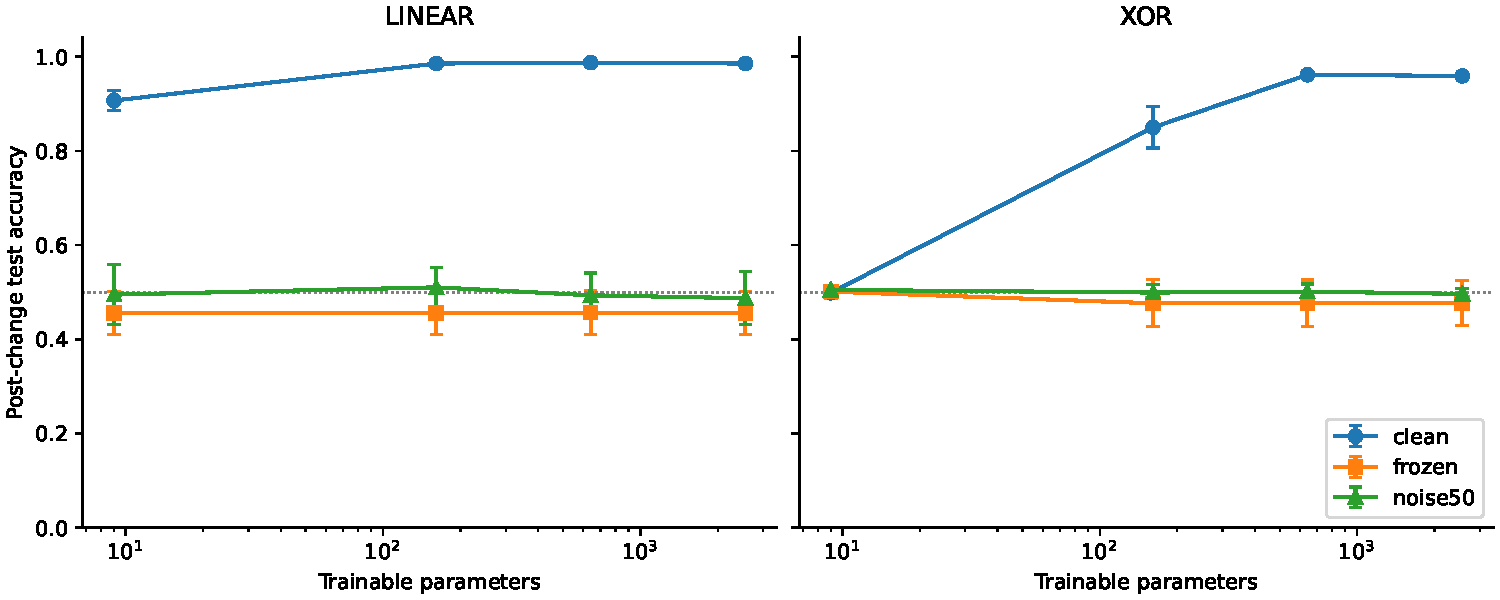
\includegraphics[width=\textwidth]{results/study-a-v2/capacity-feedback.pdf}
\caption{Capacity and feedback jointly determine observed accuracy. Error
bars are descriptive 95\% t intervals across 20 seeds. The dotted line is
chance accuracy; noisy feedback can coexist with information retained from
warmup, so individual noisy outcomes need not equal chance.}
\end{figure}

At an equal adaptation arithmetic proxy, the small model's 256 updates and
the largest model's 16 updates both cost 7,077,888 proxy FLOPs. The small
model leads by 42.80 points on linear tasks and 34.72 on XOR. However, it
receives sixteen times as many new examples, while the large model's warmup
cost is sixteen times greater. This is a particular compute/information trade,
not an isolated causal effect of feedback-loop efficiency or a scaling law.

\subsection{Feedback variations, transfer, and retention}
For the 161-parameter model, clean, 25\% corruption, and 50\% corruption yield
98.53\%, 92.05\%, and 51.03\% accuracy on linear tasks and 84.97\%, 71.84\%,
and 49.92\% on XOR. Inverted feedback yields 1.20\% and 13.32\% respectively.
More updates can reinforce the wrong target when the update rule assumes
trusted labels.

Delayed feedback reaches 98.28\% and 81.87\% at the online endpoint. After
flushing, its scores and final training losses equal clean feedback for every
seed and capacity. This equality is a correctness check for ordered updates,
not an additional empirical discovery about latency.

\begin{figure}[ht]
\centering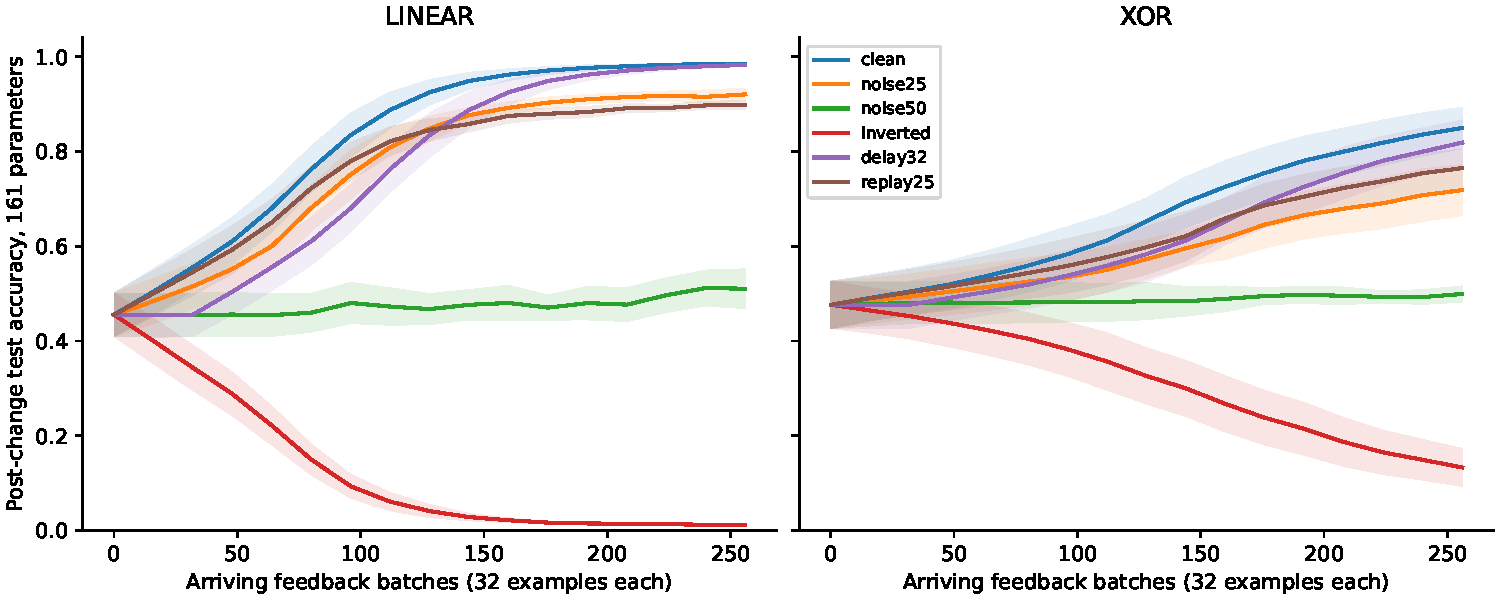
\includegraphics[width=\textwidth]{results/study-a-v2/learning-curves.pdf}
\caption{The same 161-parameter learner under six update conditions. Shading
shows descriptive 95\% seed-level intervals at fixed arrival checkpoints.}
\end{figure}

Clean small-model uniform-input accuracy is 98.44\% for linear rules and
88.19\% for XOR. This is distribution transfer within the same known rule
family, not transfer to an unrelated task. Old-rule accuracy after clean
adaptation is 45.23\% and 51.94\%. Replay raises these to 54.92\% and
64.43\% while lowering new-rule accuracy to 89.85\% and 76.48\%.
Because rules may conflict without a task identifier, this is an adaptation--
retention tradeoff; perfect performance on both is not always possible.

\subsection{Study B: feedback does not guarantee compositional gains}
\begin{table}[ht]
\centering
\caption{Study B mean constrained first-token accuracy (\%), 24 environments.
Direct tests use one command; composition tests use two. Chance is 12.5\%.}
\begin{tabular}{l r r r r r}
\toprule
Model & Direct none & Direct clean & Compose none & Compose clean & Compose oracle\\
\midrule
0.5B & 13.80 & 12.24 & 11.46 & 11.46 & 11.46\\
1.5B & 13.28 & 13.02 & 11.20 & 12.63 & 12.89\\
3B & 10.16 & 5.73 & 13.02 & 12.63 & 14.32\\
7B & 13.80 & 26.56 & 13.80 & 17.58 & 26.82\\
\bottomrule
\end{tabular}
\end{table}

For the primary 0.5B comparison, clean feedback and self-generated examples
both yield 11.46\% composition accuracy. The paired difference is 0.00 points
(95\% t CI [-1.03,1.03]; bootstrap [-0.78,1.04]). Clean-minus-none is also
0.00 points. This is a failure to demonstrate the hypothesized gain with this
mechanism, not proof that every feedback mechanism must fail.

The 7B model reaches 26.56\% on direct tasks with clean-16 examples versus
13.80\% without examples. Its composition scores are 17.58\% and 13.80\%,
respectively: a descriptive paired difference of 3.78 points (95\% CI
[0.38,7.17]). With explicit offsets, direct accuracy rises to 75.52\%, while
composition reaches 26.82\%. Representation of the instruction, inference of
the latent rule, and execution of compositions are distinct bottlenecks.

\begin{figure}[ht]
\centering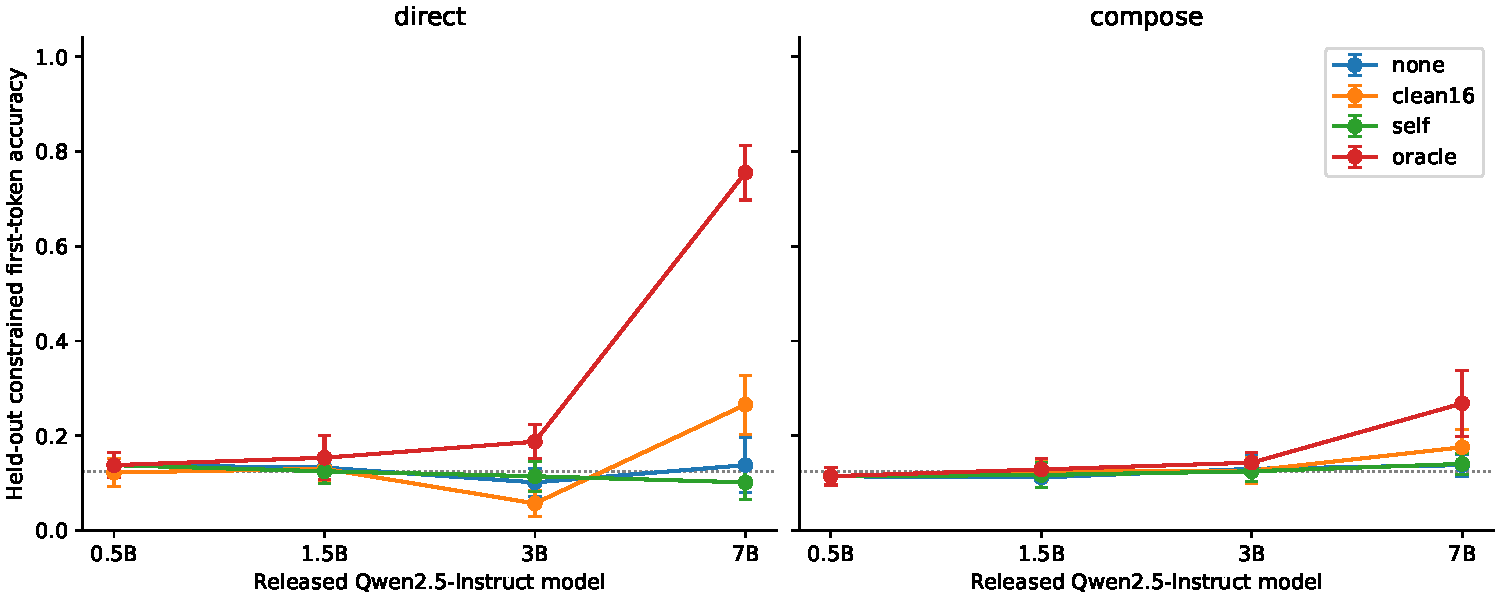
\includegraphics[width=\textwidth]{results/study-b-v1/language-model-feedback.pdf}
\caption{Released-model size and the supplied evidence affect direct and
compositional performance differently. Error bars are descriptive environment-
level 95\% t intervals. The oracle provides extra structured information;
it is not a cost-matched competitor.}
\end{figure}

LoRA trains 540,672 parameters in addition to the frozen 0.494B base. Without
example context, its direct accuracy is 26.30\% versus 13.80\% for the base.
The paired direct gain is 12.50 points (descriptive 95\% t CI [3.76,21.24]).
Composition accuracy is 13.15\%; its paired improvement over no-feedback base
is 1.69 points (95\% CI [-2.12,5.50]). Retaining examples at inference yields
13.28\% composition accuracy but reduces direct accuracy to 9.90\%.
Thus the persistent single-command gain is strongly context-dependent:
adding the same demonstrations does not preserve it. These results distinguish
a gain under the training prompt format from robust compositional transfer.

Each frozen-model suite processes 2,156,304 unpadded input tokens in 888
forward calls, including self-history construction and evaluation. Measured
suite times are 21.81, 56.22, 109.02, and 234.69 seconds; peak allocated memory
is 1.20, 3.41, 6.41, and 15.29 GiB. These figures are whole-suite accounting,
not equal lifetime budgets or per-condition causal estimates. The LoRA suite
adds 1,486,848 training input tokens and 86.67 measured update seconds. Its
extra optimization is explicitly not cost-matched to frozen inference.

\subsection{Study C: format and budget limit the generation comparison}
All 9,216 held-out predictions and 768 self-history records per model pass
source, model-revision, environment, completeness, raw-token decoding, and
score checks. Table~\ref{tab:c} reports composition accuracy; Figure~\ref{fig:c}
also shows direct predictions.

\begin{table}[htbp]
\centering\small
\begin{tabular}{llrrrr}
\toprule
Model & Interface & No examples & Clean 16 & Self & Oracle \\
\midrule
0.5B & First token & 10.68 & 11.20 & 10.68 & 10.68 \\
0.5B & Generation & 0.00 & 0.00 & 0.00 & 0.00 \\
7B & First token & 13.15 & 16.15 & 12.24 & 24.74 \\
7B & Generation & 0.00 & 6.90 & 0.26 & 97.27 \\
\bottomrule
\end{tabular}
\caption{Study C composition accuracy (\%). Generation scores include invalid
and truncated responses as defined by the frozen parser; they must be read
with the format and budget results below.}
\label{tab:c}
\end{table}

The primary 0.5B interaction is $-0.52$ percentage points (95\% t interval
[$-1.16$,0.11]; bootstrap [$-1.17$,0.00]). Its first-token clean-minus-none
effect is 0.52 points, while the generation effect is exactly zero in this
sample. Every generated answer is the literal \texttt{N} followed by EOS,
including the oracle condition. This is a failure of the tested instructions
and output interface; it cannot establish that the model lacks the reasoning
capacity measured by a different interface.

For 7B, oracle generation reaches 100\% direct and 97.27\% composition
accuracy, compared with 69.53\% and 24.74\% under first-token scoring. Thus the
narrow first-token interface can substantially understate execution capability
when the true rules are supplied. With examples, generation's clean-minus-none
composition contrast is 6.90 points (descriptive 95\% interval [4.04,9.76]),
but absolute clean accuracy falls from 16.15\% to 6.90\%. Generation improves
that contrast partly against a control with zero measured accuracy; it does
not establish a superior overall inference method.

The 128-token cap is material. In 7B composition queries, truncation rates are
100\%, 88.28\%, 95.70\%, and 0.26\% for no examples, clean examples, self
examples, and oracle offsets respectively. Corresponding invalid-format rates
are 100\%, 88.28\%, 95.57\%, and 0.26\%. A truncated response can still contain
a parseable final line, so these quantities need not coincide. Clean-example
direct generation scores 24.22\%, with 57.55\% truncation. These outcomes
leave longer-budget example induction unresolved; they are not evidence of an
unrestricted inability to infer the offsets.

Self-history also deteriorates under the interface: all 384 generated examples
for 0.5B and 354 of 384 for 7B are invalid. The resulting histories contain the
literal \texttt{invalid}, as specified. They are not 16 valid critiques or
error-directed repairs. The contrast measures the complete construction of this
self-history under the fixed prompt and budget.

Whole-suite elapsed times, excluding loading, are 28.92 and 1,831.46 seconds.
Each model uses 672 calls per interface, including history acquisition. The 7B
first-token and generation paths take 133.83 and 1,695.16 measured forward
seconds; generation emits 554,021 tokens, or 599,945 token slots with batch
padding. Such costs are recorded, not matched. All generation defaults,
including the model-specific repetition penalties, remain part of the treatment.

\begin{figure}[htbp]
\centering
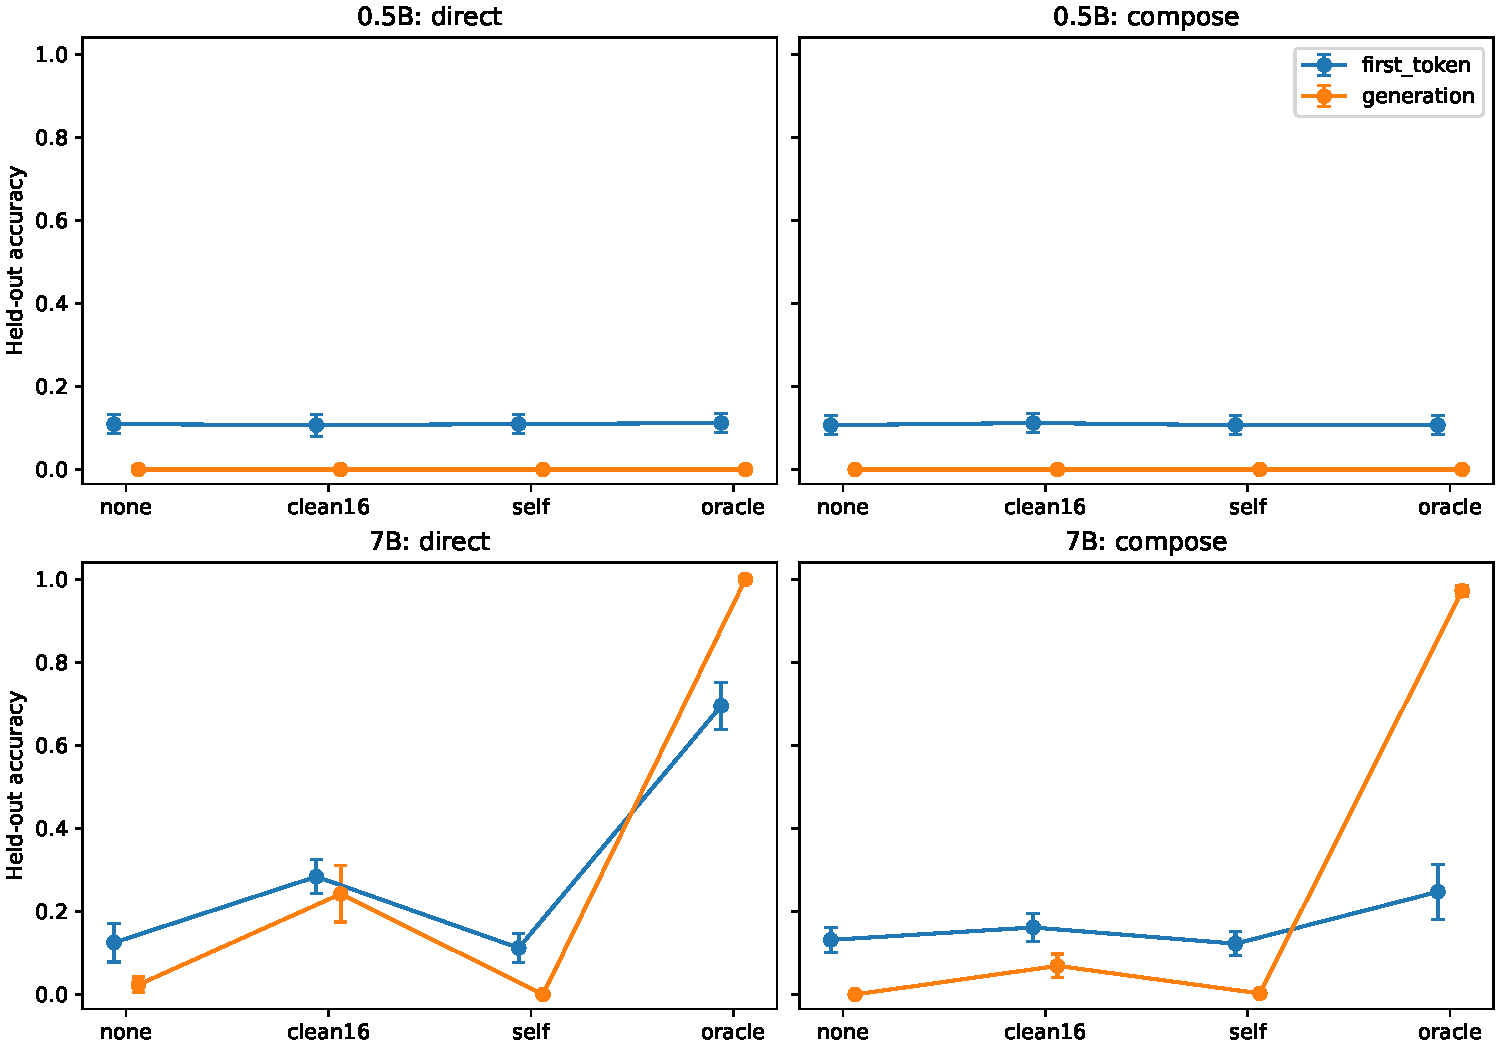
\includegraphics[width=\linewidth]{results/study-c-v1/generation-interface.pdf}
\caption{Study C response interfaces. Error bars are descriptive 95\% intervals
across 24 environment means. Strong oracle execution under generation coexists
with pervasive format or token-cap failures in other conditions.}
\label{fig:c}
\end{figure}

\subsection{Study D: longer continuations recover example-based performance}
All 3,456 continuations and 216 actual generation batches pass the registered
integrity checks. Table~\ref{tab:d} and Figure~\ref{fig:d} compare paired
prefixes on the same 24 new environments.

\begin{table}[htbp]
\centering\small
\begin{tabular}{lrrrr}
\toprule
& \multicolumn{2}{c}{Direct} & \multicolumn{2}{c}{Composition} \\
Condition & 128 tokens & 512 tokens & 128 tokens & 512 tokens \\
\midrule
No examples & 3.12 & 11.98 & 0.00 & 14.06 \\
Clean 16 & 20.05 & 59.90 & 7.94 & 70.57 \\
Oracle offsets & 100.00 & 100.00 & 96.61 & 96.88 \\
\bottomrule
\end{tabular}
\caption{Study D accuracy (\%) with fixed instructions and model. Shorter
scores use prefixes of the same deterministic continuations.}
\label{tab:d}
\end{table}

The primary clean composition difference is 62.63 percentage points (95\% t
interval [56.10,69.16]; bootstrap [56.38,68.75]). The clean-minus-none effect
at 512 tokens is 56.51 points (descriptive 95\% interval [48.99,64.03]),
compared with 7.94 at 128 tokens. The control also improves as its answers
become complete. Thus the larger budget reveals a substantial measured benefit
from the correct examples under this fixed interface.

Clean composition truncation falls from 87.76\% to 3.26\%, and invalid-format
rate falls from 87.76\% to 2.99\%. Among 768 clean composition queries, 481
change from wrong to correct and none change in the opposite direction. All
481 gains occur where the shorter prefix was invalid. Accordingly, this result
does not show correction of 481 previously valid wrong answers or isolate a
reasoning mechanism from completion of the requested answer format. It shows
that early evaluation of an unfinished response can seriously understate the
model's use of existing information. No additional environmental feedback
arrives during these continuations.

Oracle composition changes little, from 96.61\% to 96.88\%, while clean direct
accuracy rises from 20.05\% to 59.90\%. These separate direct and composition
query sets have different input lengths and generated traces; their ordering
is not a general statement that composition is easier than direct prediction.
The experiment adds no persistence across tasks, active exploration, or new
parameter updates. It neither resolves small-model format failures nor
establishes an advantage of a small learner over a large one.

The run takes 1,436.61 seconds, including 1,435.81 measured generation seconds,
processing 853,632 input tokens and 654,495 output tokens. Output padding raises
token slots to 1,044,320. The shorter prefixes have no separately measured
wall times, so these records do not support a 128-versus-512 speed ratio.

\begin{figure}[htbp]
\centering
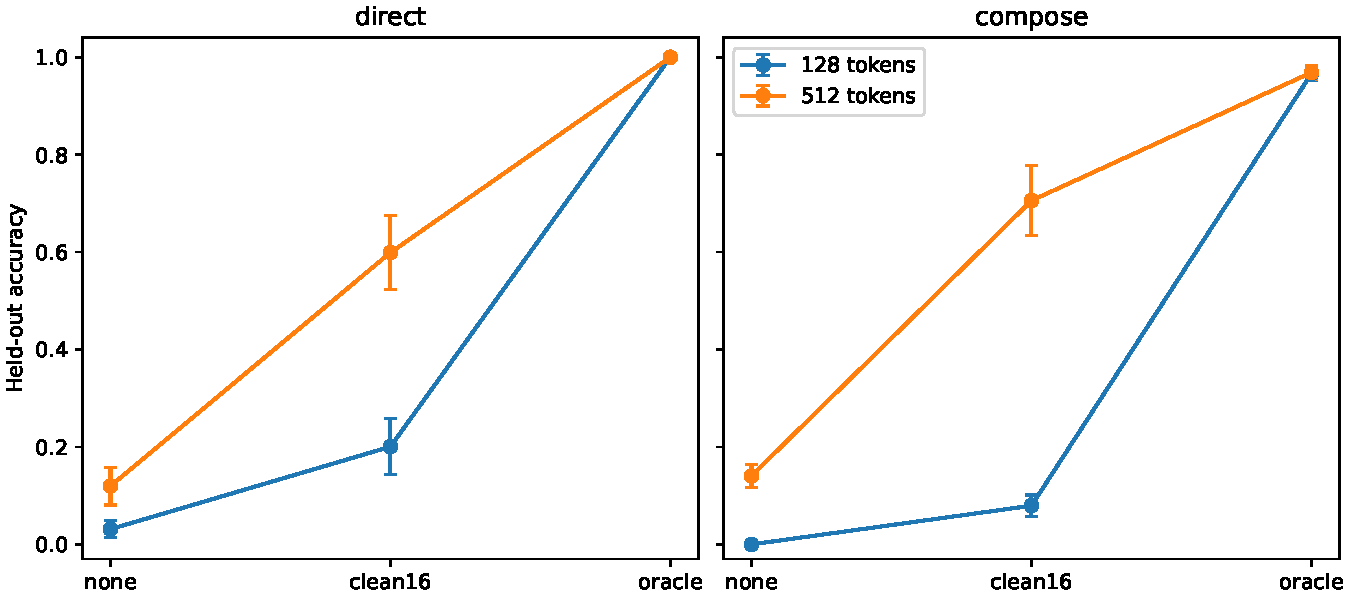
\includegraphics[width=\linewidth]{results/study-d-v1/generation-budget.pdf}
\caption{Study D generation budgets. Error bars are descriptive 95\% intervals
across 24 environment means. Extending the same continuation substantially
changes example-based accuracy; oracle execution is already nearly complete
at the shorter budget.}
\label{fig:d}
\end{figure}

\subsection{Limitations and interpretation}
All four studies use synthetic tasks with disclosed families and inexpensive
feedback. They do not measure autonomous exploration, long-horizon reward,
human intelligence, or general cross-domain skill accumulation. Study A's
fixed optimization schedule may interact with capacity. Its replay treatment
also changes fresh-example exposure. Study B uses only one model family and
a first-token response interface. Study C adds full generation but also a
strict final-line format and a fixed token cap. Study D shows that extending that cap can materially
change accuracy with the same prompt and model. Low accuracy can reflect the
interface, instruction-following ability, prior execution ability, or the
specific update schedule. None of these studies reproduces a full reflection
and error-repair agent with comparable inference-cost controls.

In development, 0.5B answered a simple arithmetic question incorrectly under
a one-digit instruction. The official weight SHA-256 matched, and CPU float32,
GPU float32/bfloat16, and eager/SDPA paths reproduced it. A subsequent ordinary
question produced the correct answer; other ordinary-language responses were
coherent. Thus the calibration reveals prompt sensitivity, not general
arithmetic incapacity. Model files and device agreement alone cannot certify
that a response interface makes full use of the available capability.

The initial Study A random-stream defect and the corrected fresh-seed
replication are both disclosed and preserved. A disk-full error occurred only
during Study B export; every original run had completion metadata and complete
predictions. Export was repeated on a separate filesystem without rerunning
models. Source hashes and complete outcome grids were checked before analysis.

Prior work already establishes reinforcement learning, external memory,
verbal reflection, and test-time computation as relevant mechanisms. Our
current evidence is a diagnostic investigation of the stated hypothesis, not
a first discovery of feedback-driven intelligence. Full-text review of six
close precedents strengthens the comparison, but a systematic novelty review
remains incomplete. External memory compression, active exploration, sustained
cross-task retention, and long-horizon reward learning remain untested.

Stability is only partially measured by Study A's old-rule retention; repeated
rule changes and long-term memory interference remain untested. Our exact
synthetic targets do not reproduce the difficulty of obtaining trustworthy
real-world feedback. No study tests reward hacking: optimizing a proxy evaluator
can improve its score without improving the intended task, particularly if the
agent can influence the feedback source. These mechanisms require separate
held-out evaluation and feedback-quality experiments; faster updates alone do
not address them.

\section{Conclusion}
Feedback enables substantial adaptation in small neural learners under task
change, but capacity remains consequential when both small and large models
learn. In the smallest pretrained model, our example-conditioning and limited
parameter-update protocols do not establish compositional improvement. Its
format failures remain unresolved. In 7B, supplying correct examples yields
substantial compositional accuracy once the continuation budget permits most
responses to finish. The earlier short-budget failures therefore cannot support
a general conclusion that this model cannot learn the disclosed rules in context.

The supported conclusion is conditional: feedback, representation, prior
learning, update rules, and response interfaces jointly determine measured
adaptation. A strong claim about small agents needs evidence of sustained
error-directed updates, retention, and transfer across diverse tasks under
comparable resource constraints. The present study establishes neither that
feedback alone explains intelligence nor that increasing model capacity is an
incorrect research direction. Its reproducible negative and positive outcomes
identify which mechanisms worked, failed, or were limited by the evaluation.

\begin{thebibliography}{11}
\bibitem{experience} D. Silver and R. S. Sutton. Welcome to the Era of Experience.
Book-chapter preprint, 2025. Author-linked copy:
\url{https://www.davidsilver.uk/publications/}.
\bibitem{silver} D. Silver, S. Singh, D. Precup, and R. S. Sutton.
Reward is enough. Artificial Intelligence, 299:103535, 2021.
\url{https://doi.org/10.1016/j.artint.2021.103535}.
\bibitem{vaswani} A. Vaswani et al. Attention Is All You Need. NeurIPS, 2017.
\url{https://arxiv.org/abs/1706.03762}.
\bibitem{kaplan} J. Kaplan et al. Scaling Laws for Neural Language Models. 2020.
\url{https://arxiv.org/abs/2001.08361}.
\bibitem{hoffmann} J. Hoffmann et al. Training Compute-Optimal Large Language Models. 2022.
\url{https://arxiv.org/abs/2203.15556}.
\bibitem{chen} H. Chen et al. Feedback is all you need: from ChatGPT to autonomous driving. 2023.
\url{https://doi.org/10.1007/s11432-023-3740-x}. Bibliographic metadata verified;
full-text argument not assessed in this version.
\bibitem{duan} Y. Duan et al. RL$^2$: Fast Reinforcement Learning via Slow Reinforcement Learning. 2016.
\url{https://arxiv.org/abs/1611.02779v2}.
\bibitem{laskin} M. Laskin et al. In-context Reinforcement Learning with Algorithm Distillation. 2022.
\url{https://arxiv.org/abs/2210.14215}.
\bibitem{shinn} N. Shinn et al. Reflexion: Language Agents with Verbal Reinforcement Learning. 2023.
\url{https://arxiv.org/abs/2303.11366v4}.
\bibitem{madaan} A. Madaan et al. Self-Refine: Iterative Refinement with Self-Feedback. 2023.
\url{https://arxiv.org/abs/2303.17651v2}.
\bibitem{huang} J. Huang et al. Large Language Models Cannot Self-Correct Reasoning Yet. ICLR, 2024.
\url{https://arxiv.org/abs/2310.01798v2}.
\bibitem{snell} C. Snell et al. Scaling LLM Test-Time Compute Optimally can be More Effective than Scaling Model Parameters. 2024.
\url{https://arxiv.org/abs/2408.03314}.
\end{thebibliography}
\end{document}
